%Ejercicio 2 (Puntos: 2)
%Ante la falta de concreción sobre todos los requisitos que el sistema debe cumplir, decides
%aplicar las metodologías ágiles durante el desarrollo y seguir Scrum en iteraciones de 2
%semanas. Para la siguiente iteración sabes que tu equipo es capaz de completar 20 puntos de
%historia y tienes la siguiente pila de trabajo (product backlog):
%-
%Historia de usuario A: 13 puntos
%-
%Historia de usuario B: 8 puntos
%-
%Historia de usuario C: 5 puntos
%-
%Historia de usuario D: 5 puntos
%-
%Historia de usuario E: 8 puntos
%-
%Historia de usuario F: 2 puntos
%A) Indica las historias de usuario que deben formar parte de la siguiente iteración (0,75 puntos) -
%0,25 puntos por cada historia identificada correctamente.
%Historia de usuario A, historia de usuario C e historia de usuario F.
%B) Dibuja el Burndown Chart para la iteración según las historias elegidas (1,25 puntos) - 0,25
%por cada línea del gráfico correctamente dibujada.
\begin{itemize}
    \item \textbf{Puntos:} 2
\end{itemize}

\begin{enunciado}
    Ante la falta de concreción sobre todos los requisitos que el sistema debe cumplir, decides aplicar las metodologías ágiles durante el desarrollo y seguir Scrum en iteraciones de 2 semanas.
    Para la siguiente iteración sabes que tu equipo es capaz de completar 20 puntos de historia y tienes la siguiente pila de trabajo (product backlog):
    \begin{itemize}
        \item Historia de usuario A: 13 puntos
        \item Historia de usuario B: 8 puntos
        \item Historia de usuario C: 5 puntos
        \item Historia de usuario D: 5 puntos
        \item Historia de usuario E: 8 puntos
        \item Historia de usuario F: 2 puntos
    \end{itemize}
    \begin{enumerate}[label=\Alph*)]
        \item Indica las historias de usuario que deben formar parte de la siguiente iteración (0,75 puntos): 0,25 puntos por cada historia identificada correctamente.
        \item Dibuja el Burndown Chart para la iteración según las historias elegidas (1,25 puntos): 0,25 por cada línea del gráfico correctamente dibujada.
    \end{enumerate}
\end{enunciado}

\begin{solucion}
    \begin{enumerate}[label=\Alph*)]
        \item Las historias de usuario que deben formar parte de la siguiente iteración son:
        \begin{itemize}
            \item Historia de usuario A (13 puntos)
            \item Historia de usuario C (5 puntos)
            \item Historia de usuario F (2 puntos)
        \end{itemize}
        Total: 20 puntos.
        \item El Burndown Chart para la iteración es el siguiente:
        \begin{center}
            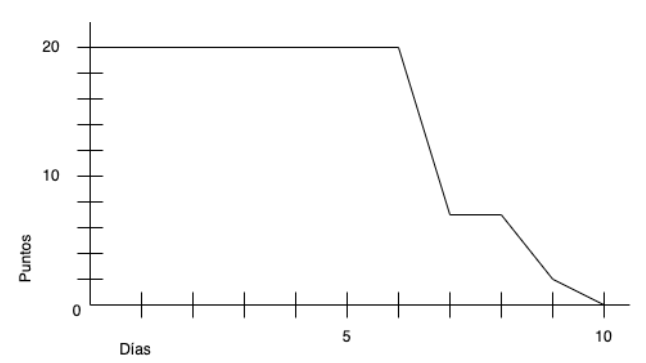
\includegraphics[width=0.8\textwidth]{../rsc/2024-ej2-bdc}
        \end{center}
    \end{enumerate}
\end{solucion}